
% 
\chapter{Implementation}
This chapter discusses the different technologies required to implement the architecture shown in figure \ref{fig:final_arch}, exploring why the technologies are an appropriate selection for the dissertation. 

\section{Applications}
To test different patterns, they require a selection of microservice based applications run under docker containers to deploy, the open-source community have built various microservice applications with different intents and features; for the purposes of testing patterns, three applications with different characteristics been chosen, allowing to simulate the different domains of microservices applications, such as a social media platform, or an e-commerce platform, making it possible to monitor effects it might have on different deployment patterns. This section further expands on the different applications and looks at their unique features and why these are a good contender for the analysis. 
\begin{figure}[H]
\begin{minipage}{.5\linewidth}
\centering
\subfloat[Social Network Architecture]{\label{fig:application_comp}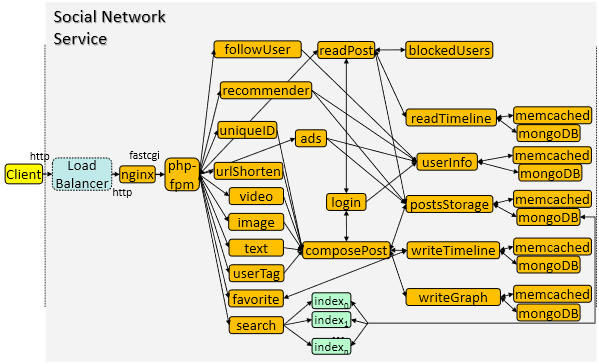
\includegraphics[scale=.4]{images/social_arch.png}}
\end{minipage}%
\begin{minipage}{.5\linewidth}
\centering
\subfloat[Hotel reservation Architecture]{\label{fig:testing_comp}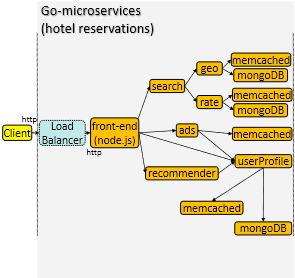
\includegraphics[scale=.53]{images/hotel_arch.png}}
\end{minipage}\par\medskip
\centering
\subfloat[Robot Shop Architecture]{\label{fig:analysis_comp}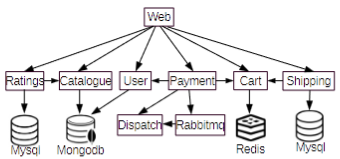
\includegraphics[scale=.65]{images/robot_shop_arch.png}}
\caption{This figure shows the different architectures for the chosen applications.}
\label{fig:application_architecures}
\end{figure}

% Talk about application features, such as number of microservice, what kinda things they look into. 
% referral links -> https://www.csl.cornell.edu/~delimitrou/papers/2019.asplos.microservices.pdf, https://www.instana.com/blog/stans-robot-shop-sample-microservice-application/, https://dl.acm.org/doi/pdf/10.1145/3297858.3304004

\textbf{Application 1: Stan’s Robot Shop}\\
\textbf{Scope:} This application is a simple e-commerce storefront based on customising and purchasing the robots and their parts. The application has been curated by developers at Instana and is to be used as a sandbox for learning orchestration and monitoring/observability techniques. \cite{Instana18}

\textbf{Functionality:} fig \ref{fig:robot_shop} shows the architecture of an end-to-end application, the front-end is a node.js server that talk's to the other services which are responsible for product catalogue, user repository, shopping cart, and order pipelines. \cite{Instana18}

\\
The following two applications are from an Open-source benchmark suite for cloud microservices, curated by the SAIL group at Cornell University. \cite{deathstar} 

\textbf{Application 2: Hotel Reservation}\\
\textbf{Scope:} This application is an online hotel reservation website, which is used for browsing information about hotels globally and making reservations, which uses the Go-microservice open-source project, and has been modified to add on backend databases, a machine learning widget used for advertisements and hotel recommendations. \cite{deathstar}

\textbf{Functionality:} fig \ref{fig:hotel_arch} shows the architecture of an end-to-end application, the front-end is a node.js server which talk's to the other services which are responsible for exploring hotel availability's in different regions and placing reservations, the back-end services use MongoDB storage for hotels and recommendations, with Memcached for caching. \cite{deathstar} 

\textbf{Application 3 : Social Network}\\
\textbf{Scope: }Social Network is an end-to-end microservice application, which implements a broadcast-style unidirectional relationships social network.  \cite{deathstar}

\textbf{Functionality:} fig \ref{fig:social_arch} shows the architecture of an end-to-end application, the front-end is a php-fqm service that talk's to the other services which are responsible for composing and displaying posts, and also the other services responsible for advertisements, search engines, etc. The messages are passed through using Apache Thrift RPC, the application also includes services for ads and recommender engines that use machine learning plugins hence. The back-end services use MongoDB storage for posts, media, profiles and recommendations, and Memcached for caching.   \cite{deathstar}


\begin{table}[H]
    
    \centering % used for centering table
    \begin{tabular}{c c c c} % centered columns (4 columns)
    \toprule\toprule %inserts double horizontal lines
     Service & Unique Microservices & Per-Language LoC Breakdown \\ [1ex] % inserts table
    %heading
    \toprule % inserts single horizontal line
    Stan's Robot Shop   & 7   & \begin{tabular}{@{}c@{}}30\% C, 21\% C++, 20\% Java, \\10\% PHP, 8\% Scala, 5\% node, 3\% Python, 3\% JS\end{tabular} \\ [2.5ex] 
    
    Hotel Reservation     & 15  & \begin{tabular}{@{}c@{}} 89\% Go, 7\% HTML, 4\% Python \end{tabular}  \\ [1.5ex]

    Social Network  & 36   &  \begin{tabular}{@{}c@{}}
    42.5\% JavaScript, 12.3\% PHP, 12.3\% Java, \\8.6\% HTML, 7.6\% Python, 7.4\% Shell
    \end{tabular}  \\ [0.5ex]

    \toprule %inserts single line
    \end{tabular}
    \caption{Characteristics and code composition of each microservices application} % title of Table\\

    \label{table:services} % is used to refer this table in the text
\end{table}


\section{Load Generators}
This section talks about the two different load generators which have been modified by the application developers to generate simulated load for the applications.

To evaluate the applications, and their behaviour behind 

(Explain why a loadd gen is needed) 



% https://dl.acm.org/doi/pdf/10.1145/3418688.3418691
% http://docs.locust.io/en/stable/what-is-locust.html#features

\textbf{Locust: }is an open-source easy use, scriptable and scalable performance testing tool. Allows for basic packet sending capabilities, and has been designed for performance testing websites and systems to test for concurrent user support. The tool runs completely on Python and allows the tester to write Locust test scripts entirely in python without adding complexity some other generators may generate load via a UI or XML files. 


\textbf{Wrk2 (Shuang's version): }




\section{Implementing Fruit Cocktail}
Fruit cocktail consists of multiple applications which are deployed with different patterns, as two patterns are to be tested, these require different directories to be created, in which these have two very similar structures however change with the terraform child modules. same structure which follows a combination of the Application Architecture and Load Architecture, as seen in the \autoref{chap:design}. 

(EXPLAIN THE TOP PARA BETTER)


The different architecture combinations, have been implemented using the various technologies described above. This section will breakdown each architectural module and talk about the various specifics in how it has been implemented before going over the integration between the two modules and analytical modules. 

\subsection{Configuration Files}
These are two files stored under an \path{artifacts} directory, the first \path{machines.txt} allows for the code to identify a list of Azure machines sizes and the other \path{units.txt} is used to identify a list of units, these units often an alphanumeric word or letter are used to track and create multiple machines with their dependencies on Azure.

\subsection{Main Architecture}
Since Terraform is an infrastrcure as code platform and does not allow to pull metrics off the cloud or initialize multiple scrpits, a bash script has been used to..

\subsection{Application Component}
With-in the architectures working directory a root module \path{main.tf} reads the \path{units.txt}, creating a list of units through local values, which allows repetitive use within the module. Next the root module uses an \path{application} block to call for a child module which is sourced locally from \path{/modules/services/application}, this child module stores the different resource blocks which describes the infrastructure objects collectively used by Azure to create the virtual machines in the cloud. 

The use of a child module with local values, allows for terraform to create 

\begin{lstlisting}[ float, caption={caption here}, label=lst:callahan]
  
locals {
 ips = split("\n", file("../artifacts/units.txt"))
}
...
module "application_a" {
  source = "../modules/services/application"

  for_each = toset( local.ips )
  unit_name = each.value
  ...
}

\end{lstlisting}

\subsection{Testing Component}

\subsection{Data Analytical Component}
Juypter notebooks take a part in this architecture as they allow to create reproducible notebooks for different tests, whilst keeping Independence from each test and making it easier to distinguish from each other. (?)

Once the files have been saved these are then organized in a new directory which can be read

% What did you do to implement this idea, and what technical achievements did you make?
% \section{Guidance}
% You can't talk about everything. Cover the high level first, then cover important, relevant or impressive details.



% \section{General points}

% These points apply to the whole dissertation, not just this chapter.



% \subsection{Figures}
% \emph{Always} refer to figures included, like Figure \ref{fig:relu}, in the body of the text. Include full, explanatory captions and make sure the figures look good on the page.
% You may include multiple figures in one float, as in Figure \ref{fig:synthetic}, using \texttt{subcaption}, which is enabled in the template.



% % Figures are important. Use them well.
% \begin{figure}
%     \centering
%     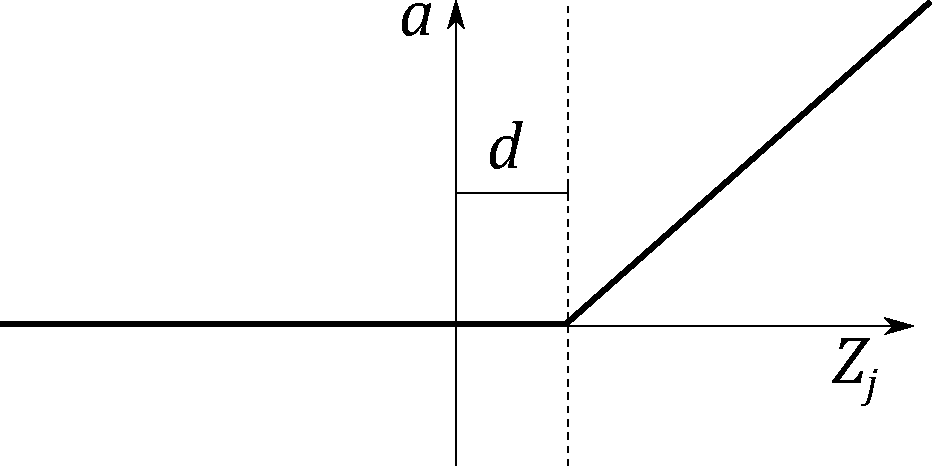
\includegraphics[width=0.5\linewidth]{images/relu.pdf}    

%     \caption{In figure captions, explain what the reader is looking at: ``A schematic of the rectifying linear unit, where $a$ is the output amplitude,
%     $d$ is a configurable dead-zone, and $Z_j$ is the input signal'', as well as why the reader is looking at this: 
%     ``It is notable that there is no activation \emph{at all} below 0, which explains our initial results.'' 
%     \textbf{Use vector image formats (.pdf) where possible}. Size figures appropriately, and do not make them over-large or too small to read.
%     }

%     % use the notation fig:name to cross reference a figure
%     \label{fig:relu} 
% \end{figure}


% \begin{figure}
%     \centering
%     \begin{subfigure}[b]{0.45\textwidth}
%         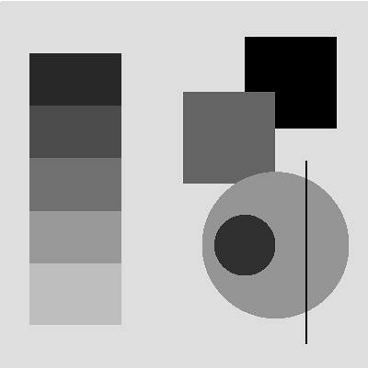
\includegraphics[width=\textwidth]{images/synthetic.png}
%         \caption{Synthetic image, black on white.}
%         \label{fig:syn1}
%     \end{subfigure}
%     ~ %add desired spacing between images, e. g. ~, \quad, \qquad, \hfill etc. 
%       %(or a blank line to force the subfigure onto a new line)
%     \begin{subfigure}[b]{0.45\textwidth}
%         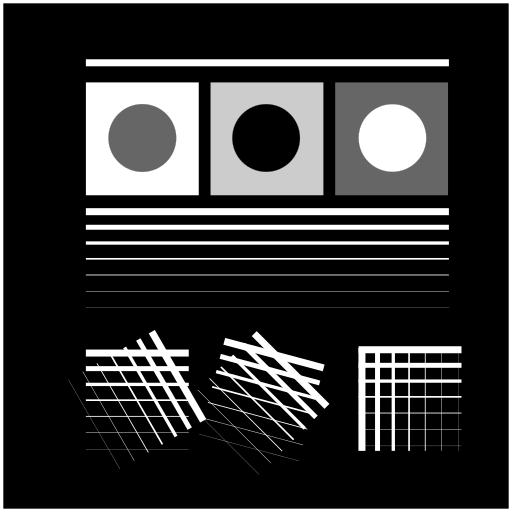
\includegraphics[width=\textwidth]{images/synthetic_2.png}
%         \caption{Synthetic image, white on black.}
%         \label{fig:syn2}
%     \end{subfigure}
%     ~ %add desired spacing between images, e. g. ~, \quad, \qquad, \hfill etc. 
%     %(or a blank line to force the subfigure onto a new line)    
%     \caption{Synthetic test images for edge detection algorithms. \subref{fig:syn1} shows various gray levels that require an adaptive algorithm. \subref{fig:syn2}
%     shows more challenging edge detection tests that have crossing lines. Fusing these into full segments typically requires algorithms like the Hough transform.
%     This is an example of using subfigures, with \texttt{subref}s in the caption.
%     }\label{fig:synthetic}
% \end{figure}

% \clearpage

% \subsection{Equations}

% Equations should be typeset correctly and precisely. Make sure you get parenthesis sizing correct, and punctuate equations correctly 
% (the comma is important and goes \textit{inside} the equation block). Explain any symbols used clearly if not defined earlier. 

% For example, we might define:
% \begin{equation}
%     \hat{f}(\xi) = \frac{1}{2}\left[ \int_{-\infty}^{\infty} f(x) e^{2\pi i x \xi} \right],
% \end{equation}    
% where $\hat{f}(\xi)$ is the Fourier transform of the time domain signal $f(x)$.

% \subsection{Algorithms}
% Algorithms can be set using \texttt{algorithm2e}, as in Algorithm \ref{alg:metropolis}.

% % NOTE: line ends are denoted by \; in algorithm2e
% \begin{algorithm}
%     \DontPrintSemicolon
%     \KwData{$f_X(x)$, a probability density function returing the density at $x$.\; $\sigma$ a standard deviation specifying the spread of the proposal distribution.\;
%     $x_0$, an initial starting condition.}
%     \KwResult{$s=[x_1, x_2, \dots, x_n]$, $n$ samples approximately drawn from a distribution with PDF $f_X(x)$.}
%     \Begin{
%         $s \longleftarrow []$\;
%         $p \longleftarrow f_X(x)$\;
%         $i \longleftarrow 0$\;
%         \While{$i < n$}
%         {
%             $x^\prime \longleftarrow \mathcal{N}(x, \sigma^2)$\;
%             $p^\prime \longleftarrow f_X(x^\prime)$\;
%             $a \longleftarrow \frac{p^\prime}{p}$\;
%             $r \longleftarrow U(0,1)$\;
%             \If{$r<a$}
%             {
%                 $x \longleftarrow x^\prime$\;
%                 $p \longleftarrow f_X(x)$\;
%                 $i \longleftarrow i+1$\;
%                 append $x$ to $s$\;
%             }
%         }
%     }
    
% \caption{The Metropolis-Hastings MCMC algorithm for drawing samples from arbitrary probability distributions, 
% specialised for normal proposal distributions $q(x^\prime|x) = \mathcal{N}(x, \sigma^2)$. The symmetry of the normal distribution means the acceptance rule takes the simplified form.}\label{alg:metropolis}
% \end{algorithm}

% \subsection{Tables}

% If you need to include tables, like Table \ref{tab:operators}, use a tool like https://www.tablesgenerator.com/ to generate the table as it is
% extremely tedious otherwise. 

% \begin{table}[]
%     \caption{The standard table of operators in Python, along with their functional equivalents from the \texttt{operator} package. Note that table
%     captions go above the table, not below. Do not add additional rules/lines to tables. }\label{tab:operators}
%     %\tt 
%     \rowcolors{2}{}{gray!3}
%     \begin{tabular}{@{}lll@{}}
%     %\toprule
%     \textbf{Operation}    & \textbf{Syntax}                & \textbf{Function}                            \\ %\midrule % optional rule for header
%     Addition              & \texttt{a + b}                          & \texttt{add(a, b)}                                    \\
%     Concatenation         & \texttt{seq1 + seq2}                    & \texttt{concat(seq1, seq2)}                           \\
%     Containment Test      & \texttt{obj in seq}                     & \texttt{contains(seq, obj)}                           \\
%     Division              & \texttt{a / b}                          & \texttt{div(a, b) }  \\
%     Division              & \texttt{a / b}                          & \texttt{truediv(a, b) } \\
%     Division              & \texttt{a // b}                         & \texttt{floordiv(a, b)}                               \\
%     Bitwise And           & \texttt{a \& b}                         & \texttt{and\_(a, b)}                                  \\
%     Bitwise Exclusive Or  & \texttt{a \textasciicircum b}           & \texttt{xor(a, b)}                                    \\
%     Bitwise Inversion     & \texttt{$\sim$a}                        & \texttt{invert(a)}                                    \\
%     Bitwise Or            & \texttt{a | b}                          & \texttt{or\_(a, b)}                                   \\
%     Exponentiation        & \texttt{a ** b}                         & \texttt{pow(a, b)}                                    \\
%     Identity              & \texttt{a is b}                         & \texttt{is\_(a, b)}                                   \\
%     Identity              & \texttt{a is not b}                     & \texttt{is\_not(a, b)}                                \\
%     Indexed Assignment    & \texttt{obj{[}k{]} = v}                 & \texttt{setitem(obj, k, v)}                           \\
%     Indexed Deletion      & \texttt{del obj{[}k{]}}                 & \texttt{delitem(obj, k)}                              \\
%     Indexing              & \texttt{obj{[}k{]}}                     & \texttt{getitem(obj, k)}                              \\
%     Left Shift            & \texttt{a \textless{}\textless b}       & \texttt{lshift(a, b)}                                 \\
%     Modulo                & \texttt{a \% b}                         & \texttt{mod(a, b)}                                    \\
%     Multiplication        & \texttt{a * b}                          & \texttt{mul(a, b)}                                    \\
%     Negation (Arithmetic) & \texttt{- a}                            & \texttt{neg(a)}                                       \\
%     Negation (Logical)    & \texttt{not a}                          & \texttt{not\_(a)}                                     \\
%     Positive              & \texttt{+ a}                            & \texttt{pos(a)}                                       \\
%     Right Shift           & \texttt{a \textgreater{}\textgreater b} & \texttt{rshift(a, b)}                                 \\
%     Sequence Repetition   & \texttt{seq * i}                        & \texttt{repeat(seq, i)}                               \\
%     Slice Assignment      & \texttt{seq{[}i:j{]} = values}          & \texttt{setitem(seq, slice(i, j), values)}            \\
%     Slice Deletion        & \texttt{del seq{[}i:j{]}}               & \texttt{delitem(seq, slice(i, j))}                    \\
%     Slicing               & \texttt{seq{[}i:j{]}}                   & \texttt{getitem(seq, slice(i, j))}                    \\
%     String Formatting     & \texttt{s \% obj}                       & \texttt{mod(s, obj)}                                  \\
%     Subtraction           & \texttt{a - b}                          & \texttt{sub(a, b)}                                    \\
%     Truth Test            & \texttt{obj}                            & \texttt{truth(obj)}                                   \\
%     Ordering              & \texttt{a \textless b}                  & \texttt{lt(a, b)}                                     \\
%     Ordering              & \texttt{a \textless{}= b}               & \texttt{le(a, b)}                                     \\
%     % \bottomrule
%     \end{tabular}
%     \end{table}
% \subsection{Code}

% Avoid putting large blocks of code in the report (more than a page in one block, for example). Use syntax highlighting if possible, as in Listing \ref{lst:callahan}.

% \begin{lstlisting}[language=python, float, caption={The algorithm for packing the $3\times 3$ outer-totalistic binary CA successor rule into a 
%     $16\times 16\times 16\times 16$ 4 bit lookup table, running an equivalent, notionally 16-state $2\times 2$ CA.}, label=lst:callahan]
%     def create_callahan_table(rule="b3s23"):
%         """Generate the lookup table for the cells."""        
%         s_table = np.zeros((16, 16, 16, 16), dtype=np.uint8)
%         birth, survive = parse_rule(rule)

%         # generate all 16 bit strings
%         for iv in range(65536):
%             bv = [(iv >> z) & 1 for z in range(16)]
%             a, b, c, d, e, f, g, h, i, j, k, l, m, n, o, p = bv

%             # compute next state of the inner 2x2
%             nw = apply_rule(f, a, b, c, e, g, i, j, k)
%             ne = apply_rule(g, b, c, d, f, h, j, k, l)
%             sw = apply_rule(j, e, f, g, i, k, m, n, o)
%             se = apply_rule(k, f, g, h, j, l, n, o, p)

%             # compute the index of this 4x4
%             nw_code = a | (b << 1) | (e << 2) | (f << 3)
%             ne_code = c | (d << 1) | (g << 2) | (h << 3)
%             sw_code = i | (j << 1) | (m << 2) | (n << 3)
%             se_code = k | (l << 1) | (o << 2) | (p << 3)

%             # compute the state for the 2x2
%             next_code = nw | (ne << 1) | (sw << 2) | (se << 3)

%             # get the 4x4 index, and write into the table
%             s_table[nw_code, ne_code, sw_code, se_code] = next_code

%         return s_table

% \end{lstlisting}
